\label{sec:Intro}
\section{Introduction}

%When we analyze data, we might make some observations that pique our curiousity and then try to find out a reason for specific observations. 
When a data scientist analyzes spatial data (e.g., using a data visualization tool), she may {\em observe} an interesting pattern. 
%Furthermore, 
%In this paper, we present an automated framework which guides the data scientist to find spatial explanations for observations made on spatial data. The proposed framework formally represents an observation as an arithmetic relationship between queries posted on the data. 
%The proposed framework introduces a taxonomy of Observation/Explanation 
For instance, the New York City Taxi and Limousine Commission (NYC TLC)\cite{taxi2016tlc} released over 1.3 billion Yellow Cab taxi trip records in the past ten years. The Yellow Cab data has several attributes including spatial attributes such as latitude, longitude and non-spatial attributes such as tip amount and total amount for each trip. Figure~\ref{fig:yellowstats} shows the number of yellow cab trips against time for January 2016. 
An example of an observation can be: ``The number of Taxi trips in NYC on January 23, 2016, dropped drastically as compared to other days of the same month". However, the data scientist may be left clueless if they cannot find a crisp {\explanation} to such a {\fact}. 
%The sharp decline in the number of trips in the last quarter of the month is pronounced. One might be inclined to look up the date when the number of trips crashed.
\begin{figure}[htp]
	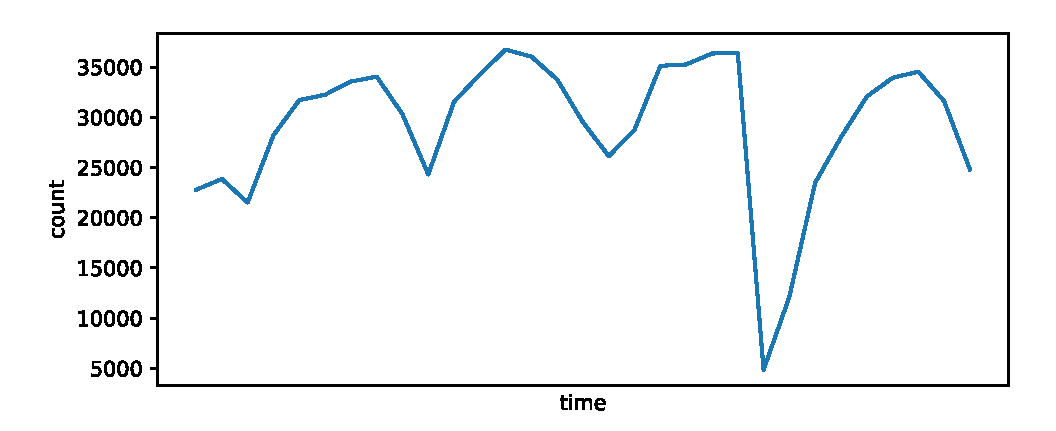
\includegraphics[width=0.9\columnwidth]{images/yellowdata_count.eps}
	\caption{Avg. \# of yellow cab trips for January 2016}
	\label{fig:yellowstats}
\end{figure}
%When we analyze data, we might make some observations that pique our curiosity. We might want to explain trends or anomalies in data.
%Without an automated system, a data analyst has to go through several manual operations to find an explanation. For small datasets, doing so might seem reasonable. 
The tedious task of finding an {\explanation} by manually scraping the data becomes even impossible with big data (e.g., NYC taxi trips).
%However, if we are dealing with a large amount of data like the NYC taxi dataset, manually finding explanations can become a tedious (or even impossible) task.% Our system is designed to produce explanations based on observations over a large amount of data. % In the past few years there has been a lot of developments in the area of Big Data.



% Since existing techniques are designed for non-spatial data, we propose a new approach for explaining spatially heterogeneous data. Our approach expands on the aggravation and intervention techniques while using spatial partitioning/clustering to improve explanations for spatial data. Experiments show that the proposed approach outperforms aggravation in precision and recall while outperforming intervention in precision when finding explanations for observations made on a real NYC taxi dataset as well as a  disease outbreak datasets.

%While some data observations might be interesting, in order to make decisions based on these observations, one might find it useful to find an explanation. For example, someone looking to start a business might look for spatial locations in which their specific category of business succeeds. It might be even more beneficial to find out why it prospers in that specific location.

%We can find several examples of decisions being made using big data analysis in everyday situations. Companies like Uber and Facebook handle large amounts of spatial data every day. Such data can be used to improve service. 
%UPS is saving millions of gallons of fuel per year using big data analytics. UPS uses On-Road Integrated Optimization and Navigation system(ORION) to determine the order of delivery, routes, and loading plans~\cite{upsarticle}.




%Given the tremendous benefits of automated analysis, the motivation for this paper was to create an automated system to help analysts answer questions about observations. The idea is to create a system which works on spatial data in general. This paper comes up with a generic system to explain observations on spatial data.




% For example, if we have taxi cab data, we might want to use this data to figure out the best locations for taxicab stands. Good locations for taxicab stands can result in less fuel consumption and lower wait times for the customers. A similar case can be made for medical emergencies and hospital locations. Even though the cost of building a hospital is much higher than that of building a taxi station, the initial cost of building the infrastructure is assuaged over time if the location is beneficial. Companies like



% In this paper, we look at different approaches to explain these types of observations. In fact, we also look at observations with a spatial dimension.

In this paper, we describe a system that automatically generates potential {\explanation}s to {\fact}s extracted from mobility datasets. The proposed approach takes two types of input. One of the inputs is the mobility dataset we want to analyze. The second input is the {\fact} observed by the data scientist. The {\fact} can be in the form of a set of aggregate queries executed on a spatial database. 
%To produce spatial explanations, the system uses one of several different solutions to find an explanation depending on what the user wants. The output of our system is an explanation for our system based on predicates.
The {\explanation}s produced by the system are parts of the data that have a significant effect on what the {\fact} data scientist is observing. %For example, assume the analyst is observing tips (given by customers in each taxi ride) for taxi trips. If removing a few tuples from the dataset has a significant impact on the average tip, then such few tuples would be considered as a potential explanation for the observation. 
Another definition of {\explanation}s in our proposed solution involves looking at different parts of the data. 
%For example, if we divide our data into a number of parts, the parts which deviate from the average value of tip percentage are considered as explanations because they introduce the largest differences.
%In this paper we extend several approaches and compare them. 
%There are three major contributions in this paper:
%\begin{itemize}


There has previously been some work related to database explanations. 
%as well as spatial analytics. 
%Since our automated framework leverages distributed computation frameworks, this section also elaborates the corresponding field. 
%The work by \cite{meliou2010causality} is a survey which looks at causality from a database perspective. Traditionally, work on causality from a database perspective mainly deals with provenance i.e. events which occurred chronologically. 
%This solution, however, only works with databases with timestamps. The paper also looks at the degree of responsibility which is defined as the number of tuples which have to be removed to change a binary observation. An example of a binary observation is winning and losing an election for instance. If a candidate wins by a high margin, each tuple has a lower degree of responsibility. On the other hand, a close victory for a candidate increases each voters degree of responsibility. 
Existing works on causality and {\explanation}s in both the Artificial Intelligence and Database communities are summarized in~\cite{meliou2014causality}. It turns out that AI problems tend to have a bigger causal network while database problems tend to have more variables.
There has also been a lot of work on correlation which shares some common ground with the work on explanations. One interesting recent work on the subject is the Data Polygamy framework \cite{chirigati2016data}. This framework is designed to find the correlation between a corpus of datasets. It uses the peaks and troughs of the data to calculate \textit{salient features} \cite{dunn1986applied}. The positive and negative correlation between these salient features can be used to decide whether datasets are related\cite{su2014supporting}. The objective of our system is a bit different from finding Correlations. There are a number of different factors which can affect {\fact}s. Correlation might be one of these attributes in certain cases. But if we ignore other criteria, such as selectivity, we might get results that do not have a significant impact. For example, if two attributes are highly correlated in a certain spatial cluster but the selectivity of the cluster is high, it would lead to a low impact on the {\fact}.




%\item We extend aggravation and intervention for spatial explanations/observations. Aggravation and Intervention techniques in literature are designed for giving non-spatial explanations for non-spatial observation. When we look at spatially heterogeneous data, the spatial context has an impact on the value of the explanations.

% \item We extend the use of salient features to give spatial explanations for simple observations based on attributes. Salient Features can be used to compare the correlation between attributes between multiple datasets. However, we repurpose the use of salient features for explanations. We use the salient features for attributes in the same dataset to form explanations.

%\item 
In this paper, we introduce a new approach: {\solution}. which employs a spatial partitioning/clustering technique to find spatial explanations for spatially heterogeneous data. Our solution is inspired by the work \cite{roy2014formal}, which outlines a formal approach to explain data. The main solutions outlined in that work are Aggravation and Intervention. However, the work by \cite{roy2014formal} is designed to work with non-spatial datasets. One of the main points of the paper is that their approach works on a dataset which can span several tables related by primary and foreign keys. While the approach outlined by \cite{roy2014formal} is great for non-spatial data, it does not translate well in the spatial domain. 
%This approach develops on previous work in causality and influence. 
It also resembles data mining concepts related to association rule mining \cite{agarwal1994fast,tan2006introduction}. 
%In association rule mining sets of attributes that occur together are assigned support and confidence. The support measures the frequency of occurrence of a set of attributes while confidence measures how frequently an attribute occurs with another set of attributes. The work by \cite{koperski1995discovery} looks at association rule mining in a spatial context. Given a set of spatial relationships, it applies association rule mining to find relationships that frequently occur together. 
There is a difference between association rule mining and our proposed approach. First of all, our proposed approach uses a user-defined observation. Secondly, in our approach, we are not looking at the associations but rather at the effect of removing or filtering pieces of data. A high association between predicates does not necessarily mean that removing them will significantly affect the {\fact}.


%for different dimensions of spatial explanations. Therefore, we propose a new approach which uses a spatial hierarchy. This accounts for explanations for multiple dimensions of the data.
%\item 
We introduce a method to balance influence and intensity to give better {\explanation}s. Influence and Intensity measure the global and local impact of an explanation, respectively. We acknowledge that the user of our system can have a non-binary preference for either. We construct our system in a way that it produces explanations as a linear relationship between influence and intensity.
%\item 
%We introduce an automated system for giving explanations based on our findings. The system that we have defined has a lot of parameters. It requires observations, coefficients, arithmetic relationships and selectivities as parameters.
%\end{itemize}


% In this thesis we define a taxonomy(Section~\ref{sec:taxonomy}) for observations and explanations.  The observation we made in Fig.\ref{fig:yellowstats} can be considered as a non spatial observation. Its explanation can either be non spatial or spatial. The first class in our taxonomy deals with non spatial explanations for non spatial observations(Section~\ref{sec:nonspatial_nonspatial}). The second class is related to spatial explanations for non spatial observations(Section~\ref{sec:spatial_nonspatial}) while the last class is about spatial explanations for spatial observations. Many geospatial datasets that we encounter contain time as one of the attributes. When we talk about spatial explanations, we do not take time into consideration. Instead, time is considered as a non-spatial attribute.

% There are three main approaches to explanation that we study in this thesis. Each approach has been extended to satisfy our taxonomy. Each approach relies on the fact that the observation is an aggregated attribute in our data set while the explanation is a predicate. \textbf{Aggravation}(Section~\ref{sec:aggravation}) is based on the principle that if we consider only the tuples in our database satisfying our explanation predicate, the value of the observation on our modified dataset will be our measure of aggravation\cite{roy2014formal,meliou2014causality}.

% In contrast, \textbf{Intervention}(Section~\ref{sec:intervention}) measures the influence of our explanation i.e. what will be the value of our observation when all the tuples satisfying our explanation predicate are removed\cite{roy2014formal}. We also extend Intervention to introduce \textbf{Hierarchical Intervention}(Section~\ref{sec:hei_intervention}). This approach measures the value of intervention when the explanation consists of a cluster of spatial polygons in our explanation predicate.

% Finally, \textbf{Salient Features}(Section~\ref{sec:salient_features}) can be used to find explanations\cite{chirigati2016data}. Each salient feature encapsulates a polygon where an attribute in the dataset is pronounced. The correlation between a salient feature of the observation and the salient feature of the explanation can give us possible explanations.

% Each approach has its own set of advantages and disadvantages. While one approach might give us very specific explanations that show a textbook example of our observation, another might give us an explanation which is hard to see in the context of the observation but has a large overall impact on it. One of the objectives of this paper is to compare which approach is suitable considering its context.

% We implemented(Section~\ref{sec:implementation}) these approaches, including hierarchical intervention using distributed data frameworks\cite{borthakur2007hadoop,dean2008mapreduce,shanahan2015large,zaharia2016apache}. We made optimizations in our implementation to make sure our approach is orders of magnitude faster than the naive approach. The implementation of salient features was used from the Data Polygamy framework \cite{chirigati2016data}.
% In order to compare each approach, we defined a few evaluation metrics. The \textbf{Intensity}(Section~\ref{sec:intensity}) metric measures how relevant each explanation is to the observation. To be more specific, it measures the value of the observation for the top explanations for each approach. The \textbf{Influence}(Section~\ref{sec:influence}) metric measures the observation when the top explanation is removed from the data. We also compare the speed(Section~\ref{sec:speed}) of our implementations of each approach.



% The approaches that we mention in his paper borrow from previous work on explanation and correlation. We have extended existing frameworks to work on our specific taxonomy. Aggravation(Section~\ref{sec:aggravation}) and Intervention(Section~\ref{sec:intervention}), for instance, are approaches which are originally designed to work in a non spatial context. They provide explanations in the form predicates over attributes. If we have a dataset with latitude and longitude as the spatial attributes, they may provide explanation in terms of just a latitude or longitude as separate continuous attributes. They might even provide explanations with no spatial attributes at all. Another drawback of using these approaches with spatial data is that they function without any knowledge of spatial locality.
%
% We highlight a new approach called hierarchical intervention (Section~\ref{sec:hei_intervention}). This approach intends to use clusters of spatially co located points or polygons in an attempt to come up with better explanations. As the name suggests, this approach borrows from the intervention approach. It uses spatial partitioning to improve spatial explanations.
%
% Another contribution of this paper is outlining a method for using salient features for explanations. The salient features approach is originally intended to work for correlation between datasets. Our extension of this approach intends to use it for the purpose of explanations. Extending salient features for explanation rather than correlation involves some additional step of work while discarding parts of the previous work which relates specifically to correlation. The original work uses salient features to compare multiple datasets and rank the most correlated datasets. Our usage of salient features is intended to explain only a single dataset with multiple attributes. Even if two attributes of a dataset are highly correlated, it may or may not rank the two attributes in the top explanations depending on the observation.

%We compare the different approaches in this paper. In order for us to compare different things, we need to do so on the basis of a common standard. The different solutions to the explanation problem are structurally very different from each other. As previously mentioned, some of them are originally not designed to handle spatial data. We have designed a common taxonomy to compare all these different solutions. On top of designing this taxonomy, our extension of each approach is designed to make sure each solution adheres to the taxonomy. Even though, this still leaves room for differences between each solution, it gives us room for comparison.

%We also define a number of evaluation metrics and an approach which uses them to come up with better explanations.
